\documentclass[tikz,border=7pt]{standalone}
\begin{document}
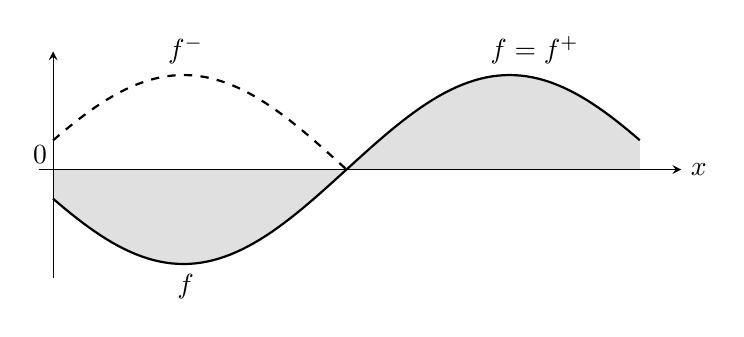
\begin{tikzpicture}[x=1.38cm,y=1.2cm,>=stealth]
  \fill[black!12] (0,0)
    -- plot[domain=0:2.7,samples=55] (\x,{sin(60*(\x-2.7))})
    -- cycle;
  \fill[black!12] (2.7,0)
    -- plot[domain=2.7:5.4,samples=55] (\x,{sin(60*(\x-2.7))})
    -- (5.4,0) -- cycle;

  \draw[->,thin] (-0.13,0) -- (5.78,0) node[right] {$x$};
  \draw[->,thin] (0,-1.15) -- (0,1.25);
  \node[above left,inner sep=2pt] at (0,0) {$0$};

  \draw[thick]
    plot[domain=0:5.4,samples=100] (\x,{sin(60*(\x-2.7))});
  \draw[thick,dashed]
    plot[domain=0:2.7,samples=55] (\x,{-sin(60*(\x-2.7))});
  \node[above] at (1.22,1.01) {$f^-$};
  \node[below] at (1.22,-1.01) {$f$};
  \node[above] at (4.43,1.01) {$f=f^+$};
\end{tikzpicture}
\end{document}
